\documentclass[journal]{IEEEtran}

\usepackage{amsmath}
\usepackage{amssymb}
\usepackage{bm}
\usepackage{mathtools}
\usepackage{algorithm}
\usepackage{algorithmic}
\usepackage{booktabs}
\usepackage{graphicx}
\usepackage{subfigure}
\usepackage{cite}
\usepackage{ulem}

\hyphenation{op-tical net-works semi-conduc-tor}


\begin{document}
\title{Optimizing Top-$k$ Multiclass SVM via Semismooth Newton Algorithm}

\author{San~Zhang, Si~Li, ~\IEEEmembership{~Fellow,~IEEE}
\thanks{S. Zhang and S. Liare with the Department of Automation,Hefei University, Anhui Province, 230031, China (e-mails: {sanzhang,sili} @mails.hfut.edu.cn).}}

\markboth{Journal of \LaTeX\ Class Files,~Vol.~14, No.~8, August~2015}%
{Shell \MakeLowercase{\textit{et al.}}: Bare Demo of IEEEtran.cls for IEEE Journals}

\maketitle


\begin{abstract}
Top-$k$ performance has recently received increasingatfention in large data categories. Advances like top-$k$ multiclasssvM have consistently improved the top-$k$ accuracy. However, the key ingredient in the state-of-the-art optimization schemebased upon Stochastic Dual Coordinate Ascent (SDCA) reliesonthe sorting method which yields $O(d\log{d})$ complexifty. Inthis paper, we leverage the semismoothness of the problem andpropose an optimized top-$k$ mul ticlass SVM algorithm,whichemploys semismooth Newton algorithm for the key buildingblock to improve the training speed. Our method enjoys a localsuperlinear convergence rate in theory. In practice,experimentalresults confirm the validity. Our algorithm is 4 times fasterthan the existing method in large synthetic problems; Moreover,on real-world datasets it also shows significant improvement intraining timc.
\end{abstract}

\begin{IEEEkeywords}
Multiclass SVM,top-k error,SDCA optsimiza-tion, root finding,semismooth Newton method.
\end{IEEEkeywords}

\IEEEpeerreviewmaketitle


\section{Introduction}
\IEEEPARstart{M}{ulticlass}classification is a fundamental problemin pattern recognition and has been attracting much attention in the machine learning community \cite{Bishop2006Pattern, Hsu2002comparison, Rifkin2004In, Yuan2012Recent, Rocha2014Multiclass}. Themajor challenges posed by large-scale dataset for trainingmulticlass classifier lies not only in the data size, but also in thenumber of data categories \cite{Deng2010What, Zhou2014Learning, Russakovsky2015Imagenet}. For example, there are 1000object categories for the image classification task in ImageNetvisual recognition challenge \cite{Russakovsky2015Imagenet}. When the object classesincrease,an important issue, i.e. the overlapping categories,emerges. Many real-world classification tasks involve largenumbers of overlapping categories \cite{Cai2007Exploiting}, which lead to classambiguity. Thus,it is customary to report top-$k$ accuracyfor large-scale object recognition problems \cite{Krizhevsky2012Imagenet, Simonyan2014Very, Szegedy2015Going, He2016Deep}, wherethe top-$k$ accuracy is the fraction of test data for which thecounted correct label is among the top-$k$ predicted labels bythe model.However,all these reported top-$k$ error rates arebased on the top-1 error. Recently, Lapin et al. generalizeCrammer and Singer's Multiclass Support Vector Machine(MSVM) \cite{Crammer2001algorithmic} to top-k MSVM which leads to improvements in top-$k$ performance \cite{Lapin2015Top}, \cite{Lapin2016Loss}.Since the direct extensionof MSVM to nonconvex top-$k$ zero-one loss will encounter acomputationally intractable problem; it minimizes the surro-gate function,i.e., so-called top-$k$ hinge loss which is a tightconvex upper bound of the top-$k$ zero-one loss. Furthermore, a highly efficient SDCA procedure \cite{Zhang2015Stochastic} is proposed to solvethe optimization problem.

\section{TOP-$k$ MULTICLASS SUPPORT VECTOR MACHINE}
we first review the well-known MSVM proposed by Crammer and Singer \cite{Crammer2001algorithmic}. Given a set of $n$ instance-label pairs $(x_i, y_i), i = 1, ..., n$, where $\bm{x}_i \in \mathbb{R}^{p}$ and the associated label $y_i$ is an integer from the set $y = \{1, ..., Y\}$. Let the weight vector $w_j$ be the $j$-th column of parameter matrix $W_{p \times Y}$. Crammer and Singer's MSVM solves the following problem
\begin{equation}
	\min\limits_{{\bf{W}}}~\frac{\lambda}{2}\sum\limits_{j\in\mathcal{Y}}\Vert{\bf{w}}_j\Vert^2+\frac{1}{n}\sum\limits_{i=1}^n\ell({\bf{W}};x_i, y_i),
\end{equation}
where is referred to as the positive regularization parameter and $\ell(\cdot)$ is called the loss function of example $(x_i, y_i)$. The loss function is defined as
\begin{equation*}
	\ell({\bf{W}};\bm{x}_i,y_i)\coloneqq \max\limits_{j\in\mathcal{Y}}\{\mathbb{I}(j\ne y_i)+\langle{\bf{w}}_j-{\bf{w}}_{y_i},\bm{x}_i\rangle\},
\end{equation*}
where $\mathbb{I}(\cdot)$ is the indicator function which takesa value of one if its argument is true. Then the multiclass decision function has the form
\begin{equation*}
	\mathop{argmax}\limits_{j\in\mathcal{Y}}\langle{\bf{w}}_j, \bm{x}\rangle.
\end{equation*}
Let $e_j$ be the $j$-th unit vector in $\mathbb(R)^Y$ and 1 with ones in all elements. For every $i$, let $c_i = 1 - e_{y_i}$, and $b_i = \bf{W}^{\top{}}x_i - (\bf{W}^{\top{}}x_i)_{y_i}$. To lighten the notation we denote the $j$-th largest component of $b_i$ by $b_{[j]},i.e.,b_{[1]} \ge b_{[2]} \ge \cdot \cdot \cdot \ge b_{[Y]}$.

Thus the loss function can be rewritten as
\begin{equation*}
	\ell{b_i} = \max\{0, (c_i + b_i)_{[1]}\}.
\end{equation*} 
Recently, Lapin et al. extended the above loss function to the top-$k$ hingle loss \cite{Lapin2015Top}, \cite{Lapin2016Loss},
\begin{equation}
	\ell_k(b_i) = \max\{0,\frac{1}{k}\sum_{j=1}^k(c_j+b_j)_{[j]}\},
\end{equation}
where $1 \leq k < Y$. We show that the top-$k$ multiclass SVM can be cast as an unconstrained optimization problem
\begin{equation}
	\min\limits_{{\bf{W}}}~\frac{\lambda}{2}\sum\limits_{j\in\mathcal{Y}}\Vert{\bf{w}}_j\Vert^2+\frac{1}{n}\sum\limits_{i=1}^n\ell_k({\bf{W}};x_i, y_i)
\end{equation}

\subsection{Dual Problem of Top-k MSVM}
To solve the top-$k$ MSVM problem (3) using the SDCA framework, one may first derive its dual form. Following the notation given in \cite{Shalev-Shwartz2016Accelerated}, let $\bf{X}_i \in \mathbb{R}^{pY \times Y}$ be the matrix whose $j$-th column is $vec(x_i(e_j-e{yi})^\top{})$ and $w = vec(\bf{W})$.Then,
\begin{equation*}
	\bf{b}_i = \bf{X}_i^\top{}w.
\end{equation*}
Hence we can reformulate the primal optimization problem of top-$k$ MSVM as
\begin{equation}
	\min\limits_{w\in \mathbb{R}^{p^Y}}~P(w):=\frac{\lambda}{2}w^\top{}w+\frac{1}{n}\sum\limits_{i=1}^n\ell_k({\bf{w}};x_i, y_i)
\end{equation}
We obtain its equivalent optimization problem
\begin{align}
	\min\frac{1}{2}\Vert\alpha_i\Vert_2^2 + a^\top{}_i\alpha_i + \frac{1}{2}(1^\top{}\alpha_i)^2 \nonumber \\
	s.t. 0 \leq -\alpha_i \leq \frac{1}{k}\sum-\alpha_i \\
	\sum-\alpha_i \leq 1 \nonumber \\
	\alpha_i^{y_i} = 0 \nonumber
\end{align}
where
\begin{equation*}
	a_i = \frac{1}{\rho_i}(c_i+\bf{X}_i^\top{}\hat{w}), \rho_i = \frac{1}{n\lambda}\Vert x_i \Vert^2.
\end{equation*}
Here calculating $\bf{X}_i^\top{}\hat{w}$ still takes $O(pY^2)$ operations, which is too expensive. We reshape the vector $\hat{w}$ into a $p$-by-Y matrix $\hat{W}$. Thus the computation
\begin{equation*}
	\bf{X}_i^\top{}\hat{w} = \hat{W}^\top{}x_i - (\hat{W}^\top{}x_i)_{y_i}
\end{equation*}
takes $O(pY)$ operations. In order to avoid the heavy notation, we drop the subscript of $a_i$ and let $z = \alpha_i^{\ y_i}, s = \sum z_j$, the above optimization problem (5) can be rewritten as
\begin{align}
	\min\limits_{z,s}\frac{1}{2}\Vert z-a \Vert^2 + \frac{1}{2}s^2 \nonumber \\
	s.t. s = \sum z_j \\
	s \leq 1 \nonumber \\
	0 \leq z_j \leq s/k \nonumber
\end{align}
Once the problem (6) is solved, a sufficient increase of the dual objective will be achieved. Whilst for the primal problem, the process will lead to the update
\begin{equation}
	w = w + \frac{1}{n\lambda}\bf{X}_i(\alpha_i - \alpha_i^{old}).
\end{equation}
A pseudo-code of the SDCA algorithm for the top-$k$ MSVM is depicted as Algorithm 1. To have the first $w$, we can initialize $\alpha_i = 0$ and then $w = 0$.

\begin{algorithm}
	\caption{Stochastic Dual Coordinate Ascent Algorithm for Top-$k$ MSVM} 
	\label{alg1}
	\begin{algorithmic}[1]
		\REQUIRE $\alpha, \lambda, k, \epsilon$
		\STATE $w \leftarrow \sum_i \frac{1}{n\lambda}\bf{X}_i\alpha_i$
		\WHILE{$\alpha$ is not optimal}
		\STATE Randomly permute the training examples
		\FOR{$i = 1,\cdot\cdot\cdot, n$}
		\STATE $\alpha_i^{old} \leftarrow \alpha_i$
		\STATE Update $\alpha_i$ by solving sub-problem (6)
		\STATE $w \leftarrow w + \frac{1}{n\lambda}\bf{X}_i(\alpha_i - \alpha_i^{old})$
		\ENDFOR
		\ENDWHILE
		\ENSURE $w, \alpha$
	\end{algorithmic}
\end{algorithm}

\section{Experiments}
In this section, we first demonstrate the performance of oursemismooth Newton method on synthetic data. Then, we applyour algorithm to the top-k multiclass sVM problem to showthe efficiency compared with the existing method in \cite{Lapin2015Top}.Ouralgorithms used to solve problem are implemented in C with aMatlab interface and run on 3.1GHz Intel Xeon (E5-2687W)Linux machine with 128G of memory. The compiler used isGCC 4.8.4. Both our code and libsdca package of \cite{Lapin2015Top} ensurethe “-O3"” optimization flag is set. The experiments are carriedout in Matlab 2016a. All the implementation will be releasedpublicly on website.

\subsection{Efficiency of the Proposed Algorithm}
To investigate the scalability in the problem dimension ofour algorithm, two synthetic problems are randomly gener-ated with $d$ ranging between 50, 000 and 2,000,000. In thefirst test problem, $a_j$ is randomly chosen from the uniformdistribution $U(15,25)$ as in \cite{Cominetti2014Newtons}, \cite{Kiwiel2008Variable}. In the second test, following the setup of \cite{Lapin2015Top}, \cite{Gong2011Efficient}, data entries are sampledfrom the normal distribution $N(0,1)$. In the third syntheticproblem, aj is chosen by independent draws from uniformdistribution $U(-1,1)$. For pure comparison, we assume theproblem without the constraint $s \leq r$. Thus,the knapsackproblem which corresponds to the $s = r$ case will not occurin these synthetic problems.

We first present numerical results to investigate the scala-bility of our proposed algorithm compared with the sorting-based method for different values of $k = 1,5$,10. Fig. 1(a),1(b) and 1(c) correspond to the first, the second and the thirdtest problems respectively. They tell us that the running timesgrow linearly with the problem size for both the sorting-based method and our proposed algorithm. However, our algorithm 1 is consistently much faster than the sorting-based method. When the problem size $d \geq 2 \times 10^6$, ourproposed algorithm is 2.5 times faster in the first problem,and 4 times faster in both the second and the third problemsrespectively. In addition to the superlinear convergence, thesemismooth Newton method accesses to accurate solutions ina few iterations.Our numerical results suggest that it usuallytakes 3$\sim$5 iterations to converge.

\begin{table}[htbp]
	\centering
	\caption{Datasets used in the experimental evaluation.}
	\begin{tabular}{l | r r r r}
		\toprule  % 顶部线
		Dataset&Classes&Features&Training size&Testing size \\ 
		\midrule  % 中部线
		FMD&10&2048&500&500 \\
		News20&20&15,478&15,935&3,993 \\
		Letter&26&16&15,000&5,000\\
		INDoor67&67&4,096&5,360&1,340 \\
		Caltech101&101&784&4,100&4,100 \\
		Flowers&102&2,048&2,040&6,149 \\
		CUB&200&2,048&5,994&5,794 \\
		SUN397&397&4,096&19,850&19,850 \\
		ALOI&1,000&128&86,400&21,600 \\
		ImageNet&1,000&2,048&1,281,167&50,000 \\
		\bottomrule  % 底部线
	\end{tabular}
\end{table}

\begin{figure*}[!htb]
	\begin{tabular}{ccc}
		\begin{minipage}[t]{0.32\linewidth}
			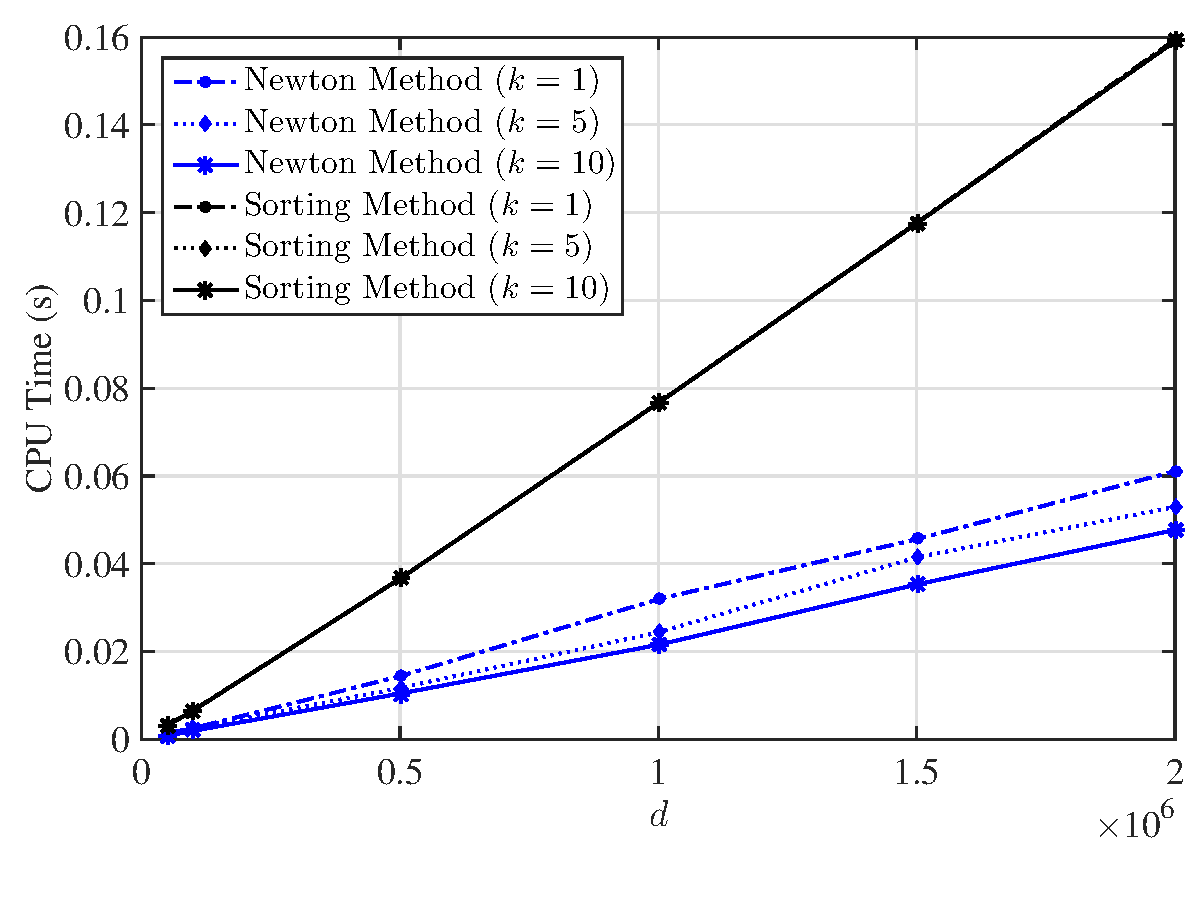
\includegraphics[width = 1\linewidth]{scale1.eps}
		\end{minipage}
	\begin{minipage}[t]{0.32\linewidth}
		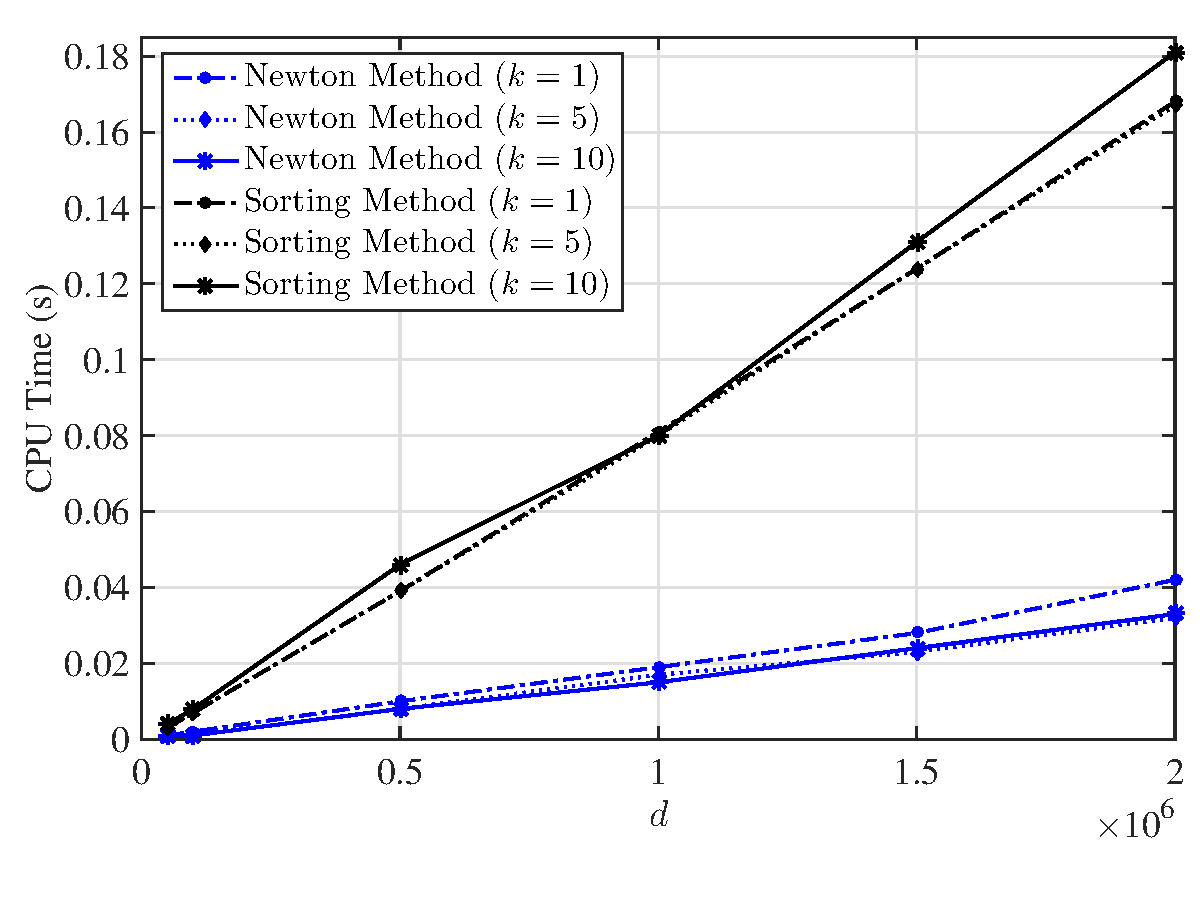
\includegraphics[width = 1\linewidth]{scale2.eps}
	\end{minipage}
		\begin{minipage}[t]{0.32\linewidth}
			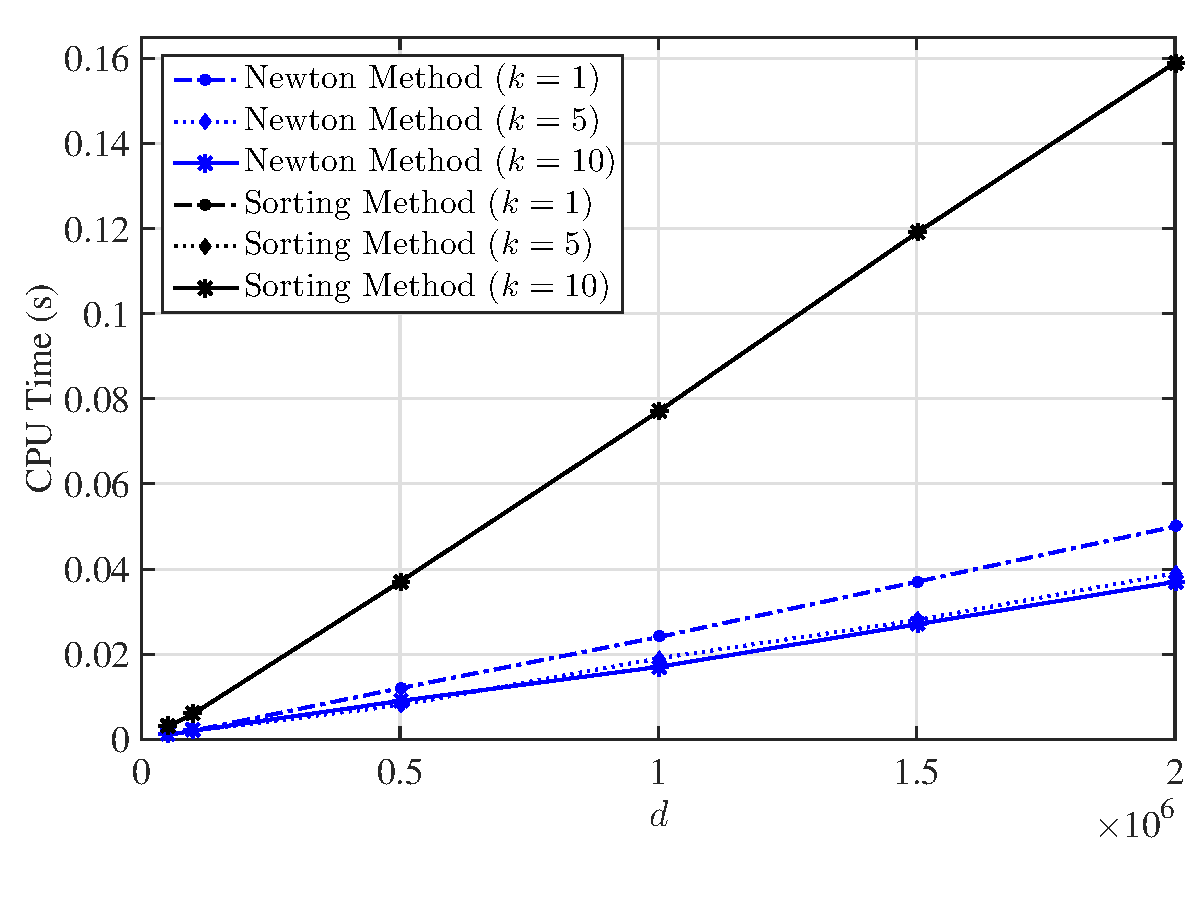
\includegraphics[width = 1\linewidth]{scale3.eps}
		\end{minipage}
	\end{tabular}
	\caption{Scaling of our algorithm compared with sorting method. Left: $a_j \sim U(10, 25)$. Middle: $a_j \sim N(0, 1)$. Right: $a_j \sim U(-1, 1)$.}     
	\label{fig}  
\end{figure*}

\section{Concluding Remarks}
In this paper, we leverage the semismoothness of the opti-mization problem and develop an optimized top-$k$ multiclass SVM. While our proposed semismooth Newton method enjoysthe local superlinear convergence rate,we also present anefficient algorithm to obtain the starting point, which worksquite well in practice for the Newton iteration. Experimentalresults on both synthetic and real-world datasets show thatour proposed method scales better with larger numbers ofcategories and offers faster convergence compared with theexisting sorting-based algorithm. We note that there are manyother semismooth scenarios, such as ReLU activation functionin deep neural networks and hinge loss in the empirical riskminimization problem. It must be very appealing to exploitthe semismooth structure and propose more efficient machinelearning algorithms in future work.

\section*{Acknowledgements}
The authors would like to thank the reviewers for their valuable suggestions on improving this paper. Thanks also goes to Wu Wang for the helpful email exchange.


\bibliographystyle{IEEEtran}
\bibliography{projection.bib}


\end{document}


